\input{src/intros/3-soap2p}

\section{Definición de Peer-to-Peer}
\label{sec:p2p_definition}

Un sistema Peer-to-Peer es un sistema distribuido de gran escala, en donde sus participantes o
nodos comparten recursos y datos entre sí de forma directa, actuando como
clientes y servidores para ello. Como gran escala se entiende que la red
contiene millones de nodos y se expande a través de internet. Schollmeier en~\cite{conf_p2p_Schollmeier01} la define de la siguiente manera:

\numberwithin{mydef}{section}
\begin{mydef}
Una arquitectura de red
distribuida puede ser llamada una red Peer-to-Peer (P-to-P, P2P, ...) si los
participantes comparten parte de sus propios recursos de hardware (poder de
procesamiento, capacidad de almacenamiento, ancho de banda, impresoras, ...).
Estos recursos compartidos son necesarios para proveer el servicio y contenido
ofrecido por la red (por. ej., compartir archivos o compartir espacios de
trabajo para colaboración). Estos son accesibles por otros nodos (o pares) en forma
directa, sin pasar por otras entidades intermediarias. Los participantes de
esta red pasan a ser tanto proveedor del recurso (servicio y contenido) como
demandante del recurso (servicio y contenido).
\end{mydef}

\section{Características de un sistema Peer-to-Peer}
\label{sec:p2p_characteristics}

De las diversas características que pueden poseer los sistema Peer-to-Peer, las
principales que idealmente debiera cumplir son:
%las que idealmente debe poseer son:
\begin{enumerate}
    \item \textbf{Escalable}: Puede crecer indefinidamente sin afectar su rendimiento.
    \item \textbf{Descentralizado}: No posee una administración central.
    \item \textbf{Heterogéneo}: Se encuentra conformado por diferentes nodos, con
diferentes características  entre sí en lo que a hardware se refiere. 
    \item \textbf{Robusto}: Se comporta bien ante caídas, pérdidas y otras
fallas de nodos de la red, manteniendo una alta disponibilidad de los datos y
servicios.
    %\item \textbf{Altamente disponible}: 
    \item \textbf{Auto-organizado}: La estructura de la red es mantenida y
organizada por los propios nodos que la conforman automáticamente, sin ninguna organización manual.
\end{enumerate}

\section{Estructura de los sistemas Peer-to-Peer}
\label{sec:p2p_estructure}

Los sistemas Peer-to-Peer se caracterizan por no poseer una coordinación
central, de tal forma que cada peer o miembro es independiente y posee una visión
local del sistema. El comportamiento global emerge de las interacciones locales
de sus miembros, y el sistema debe asegurar que toda información y servicio sea
accesible a pesar de no existir una coordinación central de la
misma~\cite{Aberer:2001:PIS:503271.503268}.
Basándose en que tan fuerte es la topología del sistema, existen sistemas Peer-to-Peer estructurados y no estructurados. Los primeros
poseen una estructura fuerte, como un árbol o un anillo, lo
cual se traduce en un costo adicional que los miembros de la red deben costear
para mantener su estructura, mientras que los segundos son simplemente un
grafo.

\subsection{Sistemas no estructurados}
\label{sec:p2p_unstructured}

\begin{figure}
\center
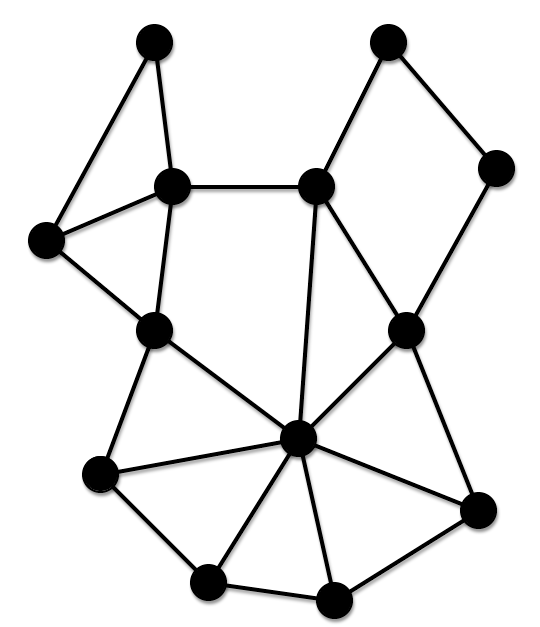
\includegraphics[width=0.5\textwidth]{img/p2p-unstructured}
\caption{Ejemplo de sistema no estructurado}
\label{fig:p2p_unstructured}
\end{figure}

%definición
Los sistemas no estructurados son aquellos que no poseen una topología con una
estructura fuerte, donde los nodos establecen enlaces entre ellos de forma
semi-arbitraria, usualmente formando grafos organizados de forma plana o jerárquica.

%ventajas
La principal ventaja de este tipo de redes es que permiten la obtención de
cierto grado de anonimato a sus usuarios.

%desventaja
La gran desventaja que posee esta topología de la red es que las búsquedas de
algún dato almacenado dentro de ella, además de tener un costo mucho mayor en lo
referente a transmisión de paquetes por la red, pueden resultar en un falso
negativo. Esto es debido a que los algoritmos de búsqueda no aseguran encontrar
el datos, porque simplemente no pasan por todos los nodos del grafo.

 %En cambio,
%en redes no-estructuradas no se puede asegurar el escrutinio completo de la
%red con una única búsqueda

Son comúnmente utilizadas para compartir archivos, aprovechando del grado de
anonimato de los usuarios para distribuir cualquier tipo de archivo por la red.

% ejemplos
Existen distintas implementaciones de sistemas no estructurados:
Gnutella~\cite{oai:CiteSeerXPSU:10.1.1.61.7302}, 
BitTorrent~\cite{bittorrent}, 
%Freenet~\cite{freenet}, 
%Overnet~\cite{overnet}, 
entre otros. Cada uno implementa diferentes
formas de organizar a los nodos, algunos generando nodos con mayor jerarquía
para facilitar las búsquedas en la red y otros simplemente no cuentan con un
sistema para realizar búsquedas (BitTorrent).

\paragraph{Almacenamiento de datos}
\label{sec:p2p_unstructured_storage}

No existe una directiva de almacenamiento de datos que tenga relación con la
topología de la red, ni un procedimiento fijo para ello. Por lo general, a medida que un nodo va solicitando
datos a la red se van generando copias del dato original, distribuyéndolo
entre más nodos de la red. Cada usuario decide si comparte un dato o no con la
red, lo que no permite controlar la densidad de un dato en la red, y por
consecuencia, su disponibilidad.
Para el apoyo de las búsquedas de la información, existen técnicas de \textit{caching} para ir
guardando la ubicación de los archivos en la red en nodos a medida que éstos son
distribuidos. 


\paragraph{Búsqueda de la información}
\label{sec:p2p_unstructured_search}
Existen diversas formas para realizar búsquedas en éste tipo de redes. Algunas
de estas son:
\begin{itemize}
    \item \textbf{Flooding}: Búsqueda en la cual cada nodo reenvía las
consultas que recibe a todos sus vecinos. Para no generar una saturación del
sistema, se utiliza un campo \textit{TTL} (Time To Live) que limita la cantidad
de veces que la misma consulta puede reenviarse. Éste tipo de búsquedas posee
un costo exponencial de mensajes por la red, de orden O($N^2)$, siendo N el
número de nodos que pueden realizar el ruteo de datos en la red.
    \item \textbf{K-Random Walk}: Búsqueda similar al caso de
\textit{flooding}. Cada nodo, al momento de reenviar la consulta, elige entre sus vecinos a un número K o porcentaje
fijo de éstos y se la reenvía a los que salieron elegidos. Una vez alcanzado un
nodo que contiene la información deseada, éste responde con un mensaje de
QUERY\_RESPONSE por el mismo camino que realizó el Random Walk, logrando
posteriormente comunicarse directamente con el nodo que originó la consulta.
El costo de mensajes que realiza la búsqueda es dependiente del valor de K,
aproximándose a: %lo indicado en~\eqref{eq:krandomwalk}.

\numberwithin{equation}{subsection}
\begin{equation}
\label{eq:krandomwalk}
 C = 2 + TTL +
\sum_{i=0}^{TTL} K^i
\end{equation}

\end{itemize}


%conclusiones
Debido a las propiedades poco favorables para la implementación de una red
social, el estudio se centrará en los sistemas Peer-to-Peer estructurados
presentados a continuación.

\subsection{Sistemas estructurados}
\label{sec:p2p_estructured}

\begin{figure}
\center
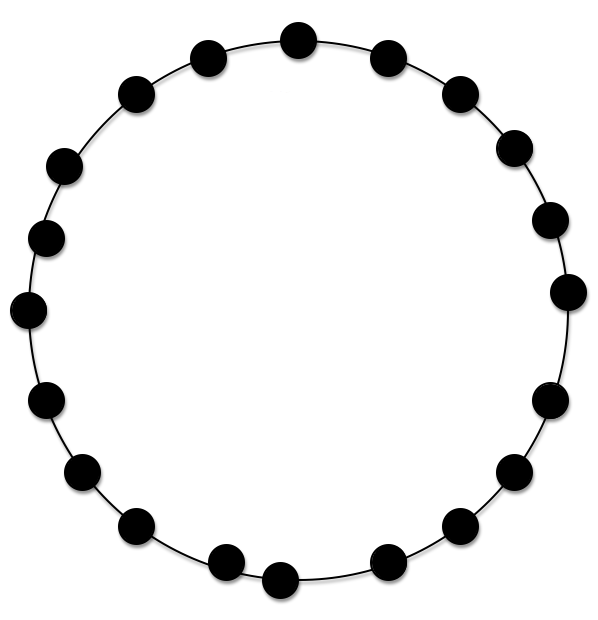
\includegraphics[width=0.5\textwidth]{img/p2p-structured}
\caption{Ejemplo de sistema estructurado}
\label{fig:p2p_estructured}
\end{figure}


%definición
Los sistemas estructurados son aquellos que poseen una topología de red
fuertemente estructurada. Mientras que la mayoría de ellos adopta topologías en
forma de anillo, otros se basan en árboles binarios y otro tipo de estructuras
para organizarse.

%ventajas
La principal ventaja de los sistemas estructurados en comparación a los no
estructurados, es que la búsqueda de datos en la red no sufre de falsos
negativos, osea que siempre va a retornar lo
que se busca si éste se encuentra en algún nodo en la red, además de ser más eficiente en
costo de mensajes y tiempo de respuesta.

%desventajas
Una de las características de las redes Peer-to-Peer estructuradas es la baja
anonimidad de los nodos pertenecientes a la red, los cuales pueden
identificarse fácilmente con una consulta desde uno de ellos. Para las
aplicaciones que desean mantener el anonimato de sus usuarios, esta es una de
los principales obstáculos para hacer uso de este tipo de redes.

% ejemplos
Gran mayoría de los sistemas Peer-to-Peer estructurados utilizan tablas de hash
distribuido (DHT)~\footnote{http://en.wikipedia.org/wiki/Distributed\_hash\_table}
como base estructural para el almacenamiento y búsqueda de los datos
almacenados por la red~\cite{BalakrishnanEtAl03}. Dentro de los sistemas que se basan en DHT, se
encuentran 
CHORD~\cite{conf:hotos:DabekBKKMSB01},
PASTRY~\cite{oai:CiteSeerPSU:441779},
OpenDHT~\cite{Rhea:2005:OPD:1080091.1080102} con Bamboo
DHT~\footnote{http://www.planet-lab.org},
entre otros.

\subsubsection{Chord}
\label{sec:chord}

Chord es un protocolo para la implementación de redes DHT que relaciona claves con nodos. Está diseñado para
funcionar en redes descentralizadas sin nodos privilegiados (es decir, sin super-nodos
que centralicen las consultas), y su funcionamiento permite obtener un resultado exhaustivo de
las búsquedas de datos que se realicen. Chord es altamente escalable, de forma que
gestiona un gran número de usuarios simultáneos sin perder rendimiento. La arquitectura
esta pensada para que dada una red con $N$ nodos, el coste de las operaciones básicas
realizadas sea proporcional a $log(N)$.

El protocolo considera una red formada por $N$ nodos que pueden estar activos o
ausentes en un momento dado. Dado un conjunto de claves
asociadas a un valor, el protocolo Chord se encarga de asignar las claves a los
nodos activos según un algoritmo y mantener esas asignaciones dinámicamente a medida
que los nodos van entrando y saliendo de la red. Utiliza como base la función
de hash consistente SHA-1 para la asignación de identificadores a los nodos y
claves del sistema.
El resto de tareas vinculadas a la red - autenticación, almacenamiento de
datos, interfaces, etc.- son responsabilidad de los implementaciones de niveles
superiores al protocolo.

\label{sec:chord}
\begin{figure}
\center
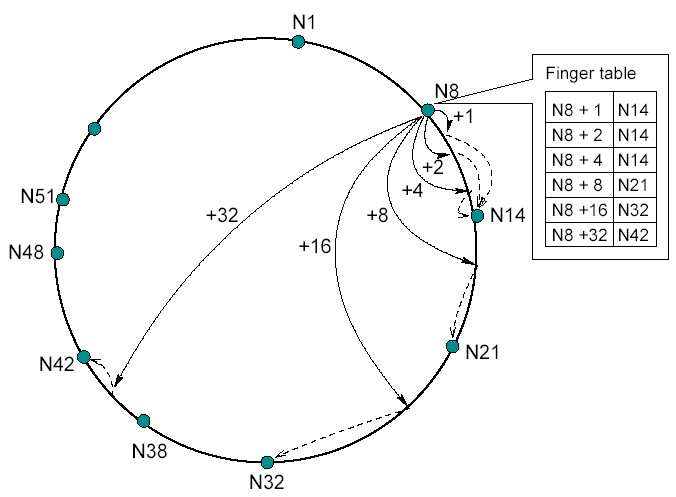
\includegraphics[width=0.5\textwidth]{img/chord-search}
\caption{Ruteo en Chord}
\label{fig:p2p_estructured_chord_search}
\end{figure}

\paragraph{Almacenamiento de datos}
 Los datos de la red son almacenados en el nodo sucesor
más cercano al hash de cada clave del dato. De ésta forma, las búsquedas en la red son
realizadas consultando a los nodos sucesores más próximos del hash que el nodo
posea en su \textit{finger table}.
De ésta forma, una clave de id $k$ se asigna al nodo de id $k$ si éste está activo en la
red. Si $k$ no se encuentra, se busca el primer nodo posterior a $k$ que esté activo y se le asigna a la
clave: este nodo sustitutivo se denomina sucesor de $k$ (successor($k$)). De
esta forma, nodos próximos físicamente pueden tener valores muy lejanos en el
espacio de claves, lo que mejora la robustez de la red.

\paragraph{Búsqueda de la información}
Chord genera pares llave-valor a través de funciones de
hashing a cada nodo participante de la red. Utiliza una tabla de enrutamiento
llamada \textit{Finger table} en donde cada nodo $\theta$ registra a $i$ nodos sucesores
de éste, cada uno correspondiendo al nodo de identificador sucesor más próximo a
$\theta + 2^(i-1)$.
 La cantidad de nodos que debe consultar para
una búsqueda es del orden $O(log(N))$. El problema que posee es que no mantiene una correlación entre el
espacio de nombres utilizado y la distancia en la red que poseen sus nodos.
Esto genera que el intercambio de mensajes entre nodos muy cercanos lógicamente
entre la red pueden sufrir de rutas físicas muy largas. Existen 
optimizaciones al protocolo a través de diferentes heurísticas,
pero ninguna resuelve completamente éste problema.

\subsubsection{Pastry}
\label{sec:pastry}
Pastry es un protocolo para la implementación de una DHT. Éste solo define como
distribuir las claves entre los nodos y como encontrar el nodo responsable de almacenar una clave.

\paragraph{Almacenamiento de datos}

El almacenamiento de datos en los sistemas estructurados tipo DHT, se realiza
aplicando la misma función de hash utilizada para asignar identificadores de
cada nodo (\textit{nodeID}), al nombre del archivo a ser almacenado. Esto resulta en una
clave, la cual es mapeada por el sistema a un único nodo. En el caso de Pastry,
este nodo posee el nodeID numéricamente más cercano a la clave del archivo.
Dicho nodo, será el encargado de almacenar el archivo.

Existen técnicas de replicación que permiten distribuir copias del archivo en
la red, haciendo que los vecinos más cercanos al nodo también guarden el
archivo. De esta forma, si el nodo que debe almacenar la información pierde
conexión, el archivo aún puede ser rescatado. Gracias al algoritmo de
asignación de los nodeID, las réplicas cercanas en la red realmente se
encuentran distribuidas lejos geográficamente, aumentando la disponibilidad de
las mismas en el sistema.

%\begin{figure}
%\center
%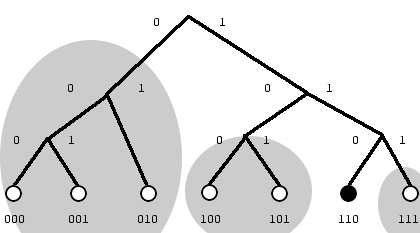
\includegraphics[width=0.65\textwidth]{img/kademlia_dht_example}
%\caption{Ejemplo de distribución del DHT en Kademlia}
%\label{fig:p2p_estructured_kademlia}
%\end{figure}

\paragraph{Búsqueda de la información}

%La búsqueda de información depende del protocolo de red utilizado.
 En el caso de Pastry, para poder buscar archivos de forma eficiente, cada nodo mantiene un
estado con tres conjuntos de información: una tabla de rutas, un conjunto
leafset y un conjunto de vecinos.
El leafset es el conjunto de nodos más próximos al nodo local en las dos
direcciones del círculo, y sirven para mantener la coherencia de la red y acortar las
búsquedas. Los nodos vecinos son los $m$ nodos más próximos según las
métricas usadas en la red, que aunque no son usados por el algoritmo de
enrutamiento, sirven para mantener la tabla de rutas.

La tabla de enrutamiento contiene una fila por cada bloque de direcciones
asignado. Los bloques se forman dividiendo el nodeID del nodo local en dígitos
de $b$ bits cada uno, generando un sistema numérico en base $2^b$. De esta forma, respecto al cliente,
agrupamos los nodos según el número de dígitos comunes en un prefijo del nodeID
del nodo local y otro nodo. La tabla almacena en cada fila la dirección del nodo conocido más
cercano y que cumple la condición del prefijo correspondiente a esa fila.

Los mensajes pueden ser dirigidos a cualquier dirección en el espacio de
claves, exista el nodo con esa ID o no. El contenido se va trasladando por al red hasta llegar al
nodo con la ID dada o, si no existe, al más próximo. Cuando un nodo recibe un mensaje para
reenviar o envía uno, consulta la tabla del leafset buscando una ruta directa. Si no la
tiene, consulta la tabla de enrutamiento buscando el nodo conocido con el mayor prefijo en
común con el objetivo, y le envía el mensaje. Esto asegura que el mensaje en cada paso vaya
a un nodo con un nodeID más cercano al destino (o en el peor de los casos, igual de cercano)
con lo que la operación converge.

% En \ref{fig:p2p_estructured_routing_table} se puede
%observar un ejemplo de la información que posee un nodo en Pastry.

%\begin{figure}
%\center
%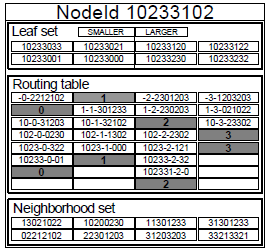
\includegraphics[width=0.4\textwidth]{img/pastry-routing-table}
%\caption{Tabla de información de ruteo de un nodo en Pastry}
%\label{fig:p2p_estructured_routing_table}
%\end{figure}

 En \ref{fig:p2p_pastry_routing} se puede
observar un ejemplo del algoritmo de enrutación de un mensaje en Pastry.

\begin{figure}
\center
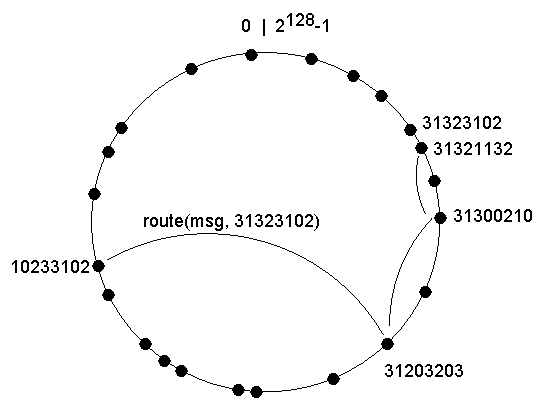
\includegraphics[width=0.6\textwidth]{img/pastryrouting}
\caption{Ruteo de un mensaje en Pastry}
\label{fig:p2p_pastry_routing}
\end{figure}


La búsqueda se basa en la función
\textit{lookup(key)}~\cite{BalakrishnanEtAl03}. Esta función, toma una
clave (\textit{key}) y busca dentro de la red un nodo cuyo nodeID es
numéricamente más cercano a la clave.  Si el dato existe en la red, la función
lookup retorna el nodo que lo posee.  Una característica importante de las
búsquedas en los DHT como Pastry, es que el costo en número de mensajes, se
mantiene en el orden $O(log(N ))$, donde $N$ es el número total de nodos en el
sistema. Además poseen la propiedad de \textit{decidibilidad}, lo cual significa
que se puede asegurar que, si un dato existe en la red, éste puede ser
encontrado en caso de ser solicitado por algún nodo. Otra característica es el
balanceo de carga que posee el sistema. El ruteo asegura
que la consulta pasará por un nodo del leafset antes de llegar al nodo raíz,
permitiendo que el nodo del leafset pueda responder a la consulta, balanceando naturalmente las
consultas entre los nodos pertenecientes al leafset del nodo raíz.



%
%
%\subsubsection{CAN}
%\label{sec:can}
%%The “Content Addressable Networks” (CAN) [22] work is being done at AT&T Center for Internet Research
%%at ICSI (ACIRI). In the CAN model, nodes are mapped onto a Æ -dimensional coordinate space on top of
%%TCP/IP in a way analogous to the assignment of IDs in Tapestry. The space is divided up into Æ dimensional
%%blocks based on servers density and load information, where each block keeps information on its immediate
%%neighbors. Because addresses are points inside the coordinate space, each node simply routes to the neighbor
%%which makes the most progress towards the destination coordinate. Object location works by the object
%%server pushing copies of location information back in the direction of the most incoming queries.
%%There are several key differences between CAN and Tapestry. In comparison, Tapestry’s hierarchical overlay
%%structure and high fanout at each node results in paths from different sources to a single destination con-
%%verging quickly. Consequently, compared to CAN, queries for local objects converge much faster to cached
%%location information. Furthermore, Tapestry’s use of inherent locality paired with introspective mechanisms
%%means it allows queries to immediately benefit from query locality, while being adaptive to query patterns
%%and allowing consistency issues to be handled at the application layer. CAN assumes objects are immutable,
%%and must be reinserted once they change their values. Finally, Tapestry node organization uses local net-
%%work latency as a distance metric, and has been shown to be a reasonable approximation of the underlying
%%network. CAN, however, like Chord, does not attempt to approximate real network distances in their topol-
%%ogy construction. As a result, logical distances in CAN routing can be arbitrarily expensive, and a hop
%%between neighbors can involve long trips in the underlying IP network. The main advantage a CAN has is
%%that because of the simplicity of the node addition algorithm, it can better adapt to dynamically changing
%%environments such as sensor networks.
%%In summary, Pastry, Chord and CAN are very similar to Tapestry in their functionality and run-time proper-
%%ties. In particular, Pastry is the closest analogy offering “locating and routing” to an object, where Chord and
%%CAN both focus on providing distributed hashtable functionality. Because Pastry controls replica placement,
%%and Chord and CAN are not optimized for large objects, Tapestry is the only system which allows the user
%%to control the location and consistency of the original data, allowing the system to manipulate and control
%%only references to the object for performance. It is also noteworthy that Tapestry and Pastry have natural
%%correlation between the overlay topology and the underlying network distance, while CAN and Chord may
%%incur high physical hop counts for every logical hop.
%
%\begin{figure}
%\center
%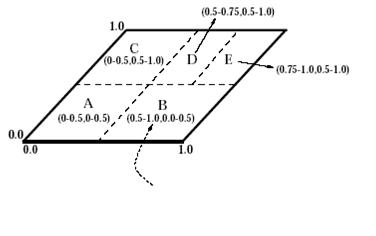
\includegraphics[width=0.6\textwidth]{img/can_structure}
%\caption{Ejemplo de la estructura de CAN}
%\label{fig:can_structure}
%\end{figure}
%
%\paragraph{Almacenamiento de datos}
%En CAN (\textit{Content Addressable Networks}) el espacio de nombres es
%dividido en bloques dimensionales~\ref{fig:can_structure} basándose en la densidad y carga de
%información de los nodos. CAN asume que los objetos son inmutables, y deben ser reinsertados
%una vez que han cambiado sus valores.
%
%\paragraph{Búsqueda de la información}
%Cada bloque mantiene información sobre sus vecinos
%inmediatos. Debido a que las direcciones son puntos dentro del espacio de
%coordenadas, cada nodo simplemente enruta hacia el vecino que realiza el mayor
%progreso frente al del vecino. Una vez que el objeto es encontrado, la
%información es enviada de forma inversa hacia la dirección de más consultas
%realizadas. Al igual que Chord, no mantiene
%correlación entre el espacio de nombres utilizado y la distancia física de los
%nodos, pero su simplicidad le permite adaptarse mejor a ambientes de alto
%dinamismo.
%
%%\subsubsection{Skip Graphs}
%%\paragraph{Almacenamiento de datos}
%%\paragraph{Búsqueda de la información}
%
%\subsubsection{Tapestry}
%\label{sec:tapestry}
%
%%PAST [11] is a recent project begun at Microsoft Research focusing on peer-to-peer anonymous storage.
%%The PAST routing and location layer, called Pastry [10], is a location protocol sharing many similarities
%%with Tapestry. Key similarities include the use of prefix/suffix address routing, and similar insertion/deletion
%%algorithms, and similar storage overhead costs.
%%There are several key differences that distinquish Pastry from Tapestry. First, objects in PAST are replicated
%%without control by the owner. Upon “publication” of the object, it is replicated and replicas are placed on
%%several nodes whose nodeIDs are closest in the namespace to that of the object’s objectID. Second, where
%
%%Tapestry places references to the object location on hops between the server and the root, Pastry assumes
%%that clients use the objectID to attempt to route directly to the vicinity where replicas of the object are kept.
%%While placing actual replicas at different nodes in the network may reduce location latency, it comes at the
%%price of storage overhead at multiple servers, and brings with it a set of questions on security, confiden-
%%tiality, and consistency. Finally, Pastry routing’s analogy of Tapestry’s “surrogate routing” algorithm (see
%%Section 3.3) provides weaker analytic bounds on the number of logical hops taken. In Tapestry, we have
%%analytically proven, well-defined, probabilistic bounds in routing distances, and are guaranteed to find an
%%existing reachable object (see Section 3).
%
%\paragraph{Almacenamiento de datos}
%Comparte muchas similitudes con Pastry, como su ruteo basado en el
%prefijo de las direcciones, algoritmos similares para la  inserción y borrado y
%costos de almacenamiento de la información.
%Tapestry usa claves numéricas de 160 bits, generadas mediante SHA-1, como
%identificadores tanto de nodos como de objetos dentro de la red. Éstos
%identificadores suelen representarse en formato hexadecimal, siendo más
%próximos dentro del espacio de identificadores contra más dígitos tengan en
%común. 
%Los objetos son publicados enviando un mensaje de publicación hacia el nodo
%raíz correspondiente al hash del objeto. Cada nodo del camino guarda un puntero
%hacia el objeto. Los links redundantes son priorizados por latencia y/o
%localidad.
%
%%De ésta forma, objetos son encontrados realizando consultas hacia la
%%raíz del objeto, en donde cada nodo por el camino revisa sus punteros y
%%redirige la petitición apropiadamente.
%
%%Participants in the network can publish objects by periodically routing a
%%publish message toward the root node. Each node along the path stores a pointer
%%mapping the object. Multiple servers can publish pointers to the same object.
%%The redundant links are prioritized by latency and/or locality. Objects are
%%located by routing a message towards the root of the object. Each node along
%%the path checks the mapping and redirects the request appropriately. The effect
%%of routing is convergence of nearby paths heading to the same destination.
%
%
%\paragraph{Búsqueda de la información}
%
%Un mensaje busca primero un nodo cercano que tenga en común con la clave
%del destino el mismo número en el dígito de menos peso, incrementando
%paulatinamente la parte común hasta encontrar el nodo existente más cercano,
%como se puede visualizar en la figura~\ref{fig:bayeux_routing}.
%
%Para dirigir los mensajes a su destino, Tapestry usa tablas de enrutamiento
%locales en cada nodo, conocidas como \textit{neighbor maps}. La tabla contiene
%múltiples niveles, en donde cada nivel representa un sufijo coincidente hasta
%un dígito. Un nivel dado contiene varias claves, las cuales varían solo en el
%número en la posición indicada por la tabla, similar a la tabla de ruteo
%utilizada por Pastry.
%
%Una búsqueda realiza $O(log_B N)$ saltos en una red de tamaño $N$ y espacio de
%nombres de base $B$. Para un mejor nivel de tolerancia de fallos, se mantiene
%una lista de $c$ links secundarios, de tal forma que la tabla de ruteo posee
%un tamaño de $c B log_B( N)$.

%\red{OTRAS REDES}
